%%________________________________________________________________________
%% LEIM | PROJETO
%% 2022 / 2013 / 2012
%% Modelo para relatório
%% v04: alteração ADEETC para DEETC; outros ajustes
%% v03: correção de gralhas
%% v02: inclui anexo sobre utilização sistema controlo de versões
%% v01: original
%% PTS / MAR.2022 / MAI.2013 / 23.MAI.2012 (construído)
%%________________________________________________________________________


%%________________________________________________________________________
\chapter{Implementação do Modelo}
\label{ch:implementacaoDoModelo}
%%________________________________________________________________________

(todo)

\section{Análise dos dados}
O processo de análise começou após a reunião inicial comm os orientadores do projeto, onde recebemos os ficheiros com que iamos trabalhar. Tratar este ficheiros implicou várias fases de análise, onde delineamos estratégias para conseguir extrair dados e possiveis gráficos. Antes de falarmos das várias fases, teremos só de estabelecer que tipos de gráficos são os indicados para as informações que queremos mostrar.

\subsection{Análise inicial da informação}
Após termos recebido os dados, fizemos uma primeira análise com o objetivo de perceber a informação recebida e os próximos passos a tomar.

No total, recebemos 30 ficheiros \gls{xlsx} que foram exportados da plataforma, correspondentes às diferentes secções da plataforma de simulação, com vários indicadores como segmentos de mercado, características de produto, vendas, entre outros. Cada ficheiro pode conter várias folhas de cálculo, organizadas por marcas, cidades entre outros marcadores.

Durante esta análise preliminar, verificámos que:
\begin{itemize}
    \item Os nomes dos ficheiros e das folhas variam, mas seguem convenções relativamente consistentes;
    \item Alguns ficheiros apresentam estruturas de dados semelhantes, mas com diferenças no nível de detalhe ou na organização das colunas;
    \item Existiam ficheiros com dados que iriam precisar de mais transformação uma vez que representavam percentagens;
    \item Dados com muito detalhe, e com várias colunas sem representação (células marcadas com "X").
\end{itemize}

Com base nesta primeira análise, concluímos que seria necessário:
\begin{itemize}
    \item Fazer uma normalização da informação recebida para garantir uma utilização consistente da aplicação;
    \item Separar os vários ficheiros possiveis em grupos, de forma a identificar dados em comum que podessemos aplicar \textit{templates} de gráfico;
    \item Guardar os dados extraídos num formato mais prático, e que permita uma filtragem dinâmica da informação carregada (de forma a faciltiar a visualização dos dados)-
\end{itemize}

Esta análise inicial permitiu-nos estabelecer as fases seguintes em relação ao tratamento que iremos dar aos vários ficheiros possiveis. Para isso, decidimos classificar a informação em várias categorias, e aplicar tipos de gráficos especificos a cada categoria, tendo assim \textit{templates} que podemos aplicar programaticamente. 

\subsection{Classificação da informação}

A análise inicial dos ficheiros fornecidos permitiu-nos perceber que, apesar da diversidade dos mesmos,  existiam padrões consistentes na estrutura. Com base nisso, tomámos a decisão de agrupar os ficheiros em \textit{buckets} ou categorias lógicas. Cada um desses grupos ficou associado a um \textit{template} gráfico específico, o que nos permite não só uniformizar a apresentação dos dados, como também automatizar o processo de transformação e visualização a partir dos ficheiros.

Os grupos definidos foram os seguintes: \textbf{simples}, \textbf{agrupado}, \textbf{balanços}, \textbf{quartis}, \textbf{setores} e \textbf{análise específica}. Vamos então descrever o significado de cada grupo e identificar o que é comum entre os gráficos pertencentes a cada um deles.

O grupo \textbf{simples} inclui ficheiros cuja estrutura é mais direta, geralmente com apenas duas colunas: uma coluna que representa uma categoria (como por exemplo empresas ou segmentos de mercado) e uma coluna numérica (como por exemplo vendas ou lucros). Nestes casos, optámos por gráficos de barras, uma vez que o objetivo principal é comparar rapidamente valores individuais entre categorias. Nos ficheiros que avaliamos, não encontramos séries temporais, pelo que não justificou gráficos de linhas. Também nesta categoria, alguns dados eram séries mais espcificas (como dados relativos a médias e medianas) mas mantinham a mesma estrutura de dados, pelo que foram classificados como \textbf{simples} mas utilizaram gráficos diferentes como gráficos de diagramas e quartis e gráficos de setores (também conhecidos como \textit{pie charts}).

O grupo \textbf{duplo} refere-se a ficheiros onde existem múltiplas séries de dados associadas à mesma categoria. Ou seja, para cada categoria, existem vários valores (ou várias séries) que precisam de ser representados lado a lado. Para estes casos, a escolha que fizemos foi apresentar gráficos de barras agrupadas, permitindo uma comparação direta entre diferentes séries de dados para a mesma categoria, e permite visualizar todos os dados relacionados com essa categoria.

O grupo \textbf{balanços} abrange ficheiros associados a balanços financeiros ou variações de stock, onde faz sentido representar aumentos e diminuições de valores ao longo de um processo ou período. Para estes ficheiros, o \textit{template} selecionado foi o gráfico de cascata (ou um gráfico \textit{financial waterfall}), dado que este tipo de visualização representa as várias componentes do valor total.

No grupo \textbf{quartis}, classificámos ficheiros onde os dados contem minimos, máximos e médias. Aqui, optámos por representar a informação através de gráficos de quartis, que são uteis para mostrar a mediana, a dispersão e possíveis valores \textit{outliers}. Para este tipo de grárfico, tentámos sempre fazer com que a leitura do mesmo seja o mais fácil possível.

O grupo \textbf{setores} inclui ficheiros onde a segmentação do mercado ou da performance está organizada por setores económicos ou geográficos. Nestes casos, faz sentido usar gráficos de setores (também conhecidos como pie charts),  dependendo da necessidade de comparar proporções entre segmentos.

Finalmente, o grupo de \textbf{análise específica} são ficheiros que não se encaixam diretamente nos formatos anteriores, como análises mais detalhadas por cidade, por segmento ou quando os dados incluem várias unidades na mesma folha (percentagens com euros). Para estes casos, o processo passou por simplificar a informação de modo a encaixar num dos grupos acima ou excecionalmente aplicar um novo tipo de gráfico, e a análise foi feita manualmente para cada caso. Para casos em que a não era possível aplicar um \textit{template} de gráfico, não foi possivel simplificar a informação e não encontrámos uma represetnação gráfica que fosse fácil de intepreta, optámos por não aplicar nenhum gráfico, e apenas apenas mostrar uma tabela interativa com os dados onde o utilizador podia filtrar os dados por diferentes colunas.


No final, dos 103 ficheiros recebidos, a classificação foi a seguinte:
\begin{figure}[h]
    \centering
    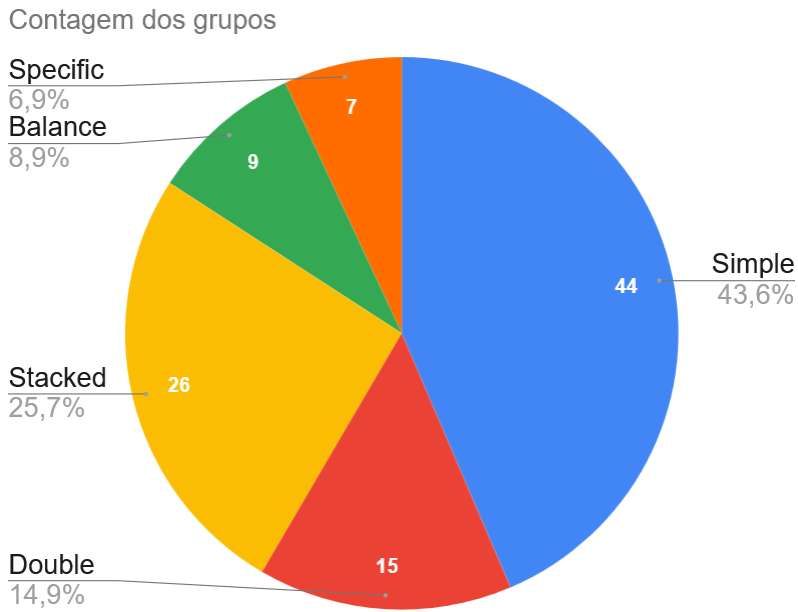
\includegraphics[width=\textwidth]{./img/stats1}
 \caption{Classificação dos ficheiros - contagem final dos grupos}
 \end{figure}

Em termos de representações utilizadas, a distribuição é a seguinte:
\begin{figure}[h]
    \centering
    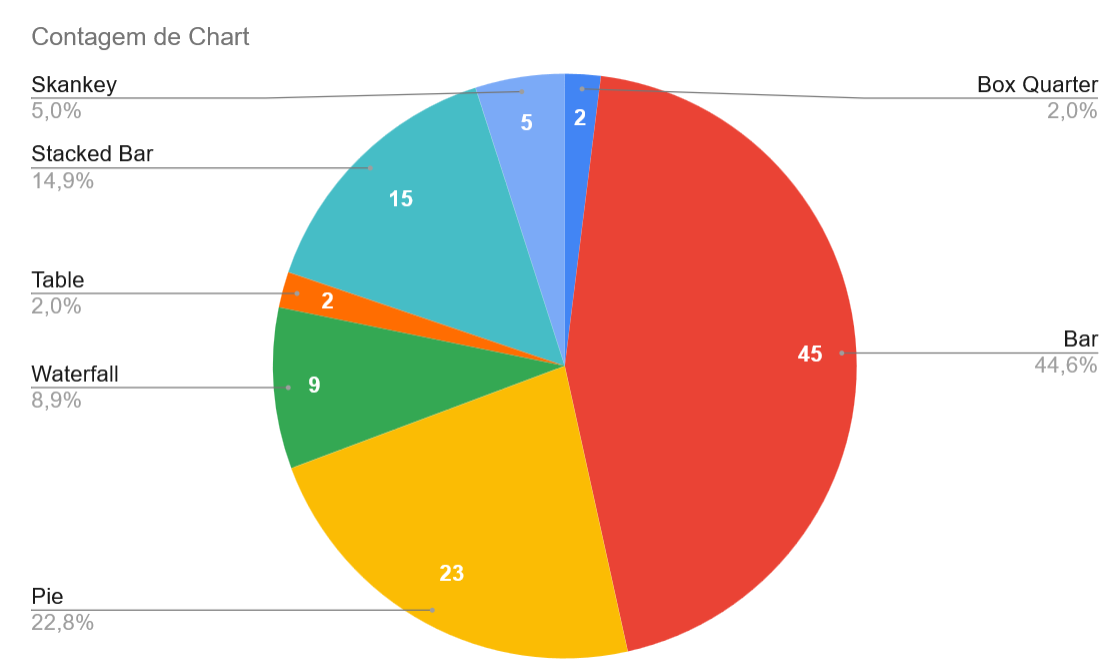
\includegraphics[width=\textwidth]{./img/stats2}
 \caption{Classificação dos ficheiros - contagem final de representações utilizadas}
 \end{figure}

\section{Processamento dos dados}
- Iniciar o tema de processamento de informação, converter informação desconhecida para um formato normalizado.
- explicar como foi feito o processamento, em que alguns ficheiros passam por várias fases


\subsection{\textit{Pipeline} de transformação dos dados}
A primeira fase de normalização segue os seguintes passos:
\begin{itemize}
    \item Extrai o nome do gráfico a partir da primeira linha de cada folha.
    \item Usa a segunda linha como cabeçalhos e normaliza os nomes (ex: substitui espaços por \textit{underscores}, remove quebras de linha).
    \item Remove colunas irrelevantes com base numa lista de columnas que não tem representação.
    \item Normaliza dados nas células (como por exemolo: remove quebras de linha, espaços duplos).
\end{itemize}

A segunda fase vai depender do ficheiro e do gráfico que queremos apresentar, mas no geral,

(...) completar isto

- Falar como foi desenvolvida, e as várias fases  de transformação A desenvolvida em \textit{Python} com recurso ao Pandas. 


\subsection{Conversão e Exportação para \gls{csv}}
- Falar sobre a transformação do pandas\n
- Falar da exportação do \gls{csv}\n
- Falar da gestão de ficheiros  \gls{csv} e \gls{xlsx}, e metodologias para não haver conflito entre ficheiros carregados\n


\section{Desenvolvimento da Aplicação Web}

Esta secção foca-se na estrutura e funcionamento da aplicação web — tanto o backend em Django como a interface construída com HTML, WebComponents e Flowbite.
\subsection{Arquitetura da aplicação Django}

    \begin{itemize}
        \item Descrever como está organizada a aplicação: os modelos principais (Quarter, ExcelFile, CSVFile), as relações entre eles e como são usados para garantir o isolamento por utilizador.
        \item Explicar o sistema de autenticação (Django Auth) e como se garantem as permissões e o acesso aos dados por utilizador.
        \item Referir também o uso do sistema de media (uploads) com UUIDs por quarter, e a criação automática das pastas.
    \end{itemize}

\subsection{Endpoints e API interna}

    Detalhar os principais endpoints utilizados: uploads, visualização de gráficos, listagem de ficheiros, etc.

    \begin{itemize}
        \item Mencionar a estrutura REST dos endpoints e como a interface os consome (por exemplo, o /api/charts/<chart_id>/<quarter>/).
        \item 
        \item Referir como se gere o estado do sistema com propriedades como \textit{is_current}, e o que acontece quando se substitui um ficheiro existente.
    \end{itemize}

\subsection{Sistema de processamento assíncrono e normalização}

    \begin{itemize}
        \item Falar sobre o \textit{run_pipeline_for_sheet}(...) do data_processing.py e como isso se encaixa com o modelo ExcelFile.
        \item 
        \item Comentar o sistema de marcação dos ficheiros como processados e o uso de flags como processed.
    \end{itemize}



    \section{Interface Gráfica e Experiência do Utilizador (Frontend)}

Aqui explicas como a interface foi pensada, as ferramentas utilizadas e como os gráficos são construídos com base nos dados enviados pelo backend.
\subsection{Design System e Flowbite}

    Explicar por que escolheste Flowbite e como ele ajudou a construir uma UI consistente e reutilizável.

    Mostrar exemplos de componentes reutilizados, como modais, botões, tabs, etc.

\subsection{WebComponents e gráficos interativos}

    Falar sobre como encapsulaste a lógica dos gráficos usando WebComponents, para evitar conflitos de JS e garantir modularidade.

    Descrever a comunicação entre os WebComponents e o backend via fetch, passando parâmetros (por exemplo, o quarter atual, ou filtros).

\subsection{Gestão de Quarters e Uploads}

    Mostrar como funciona a criação de quarters e a navegação entre diferentes trimestres (com os botões e setas).

    Explicar o fluxo de upload de ficheiros e como a interface valida o tipo de ficheiro, evita duplicações, e atualiza a visualização após carregamento.

%%________________________________________________________________________
\chapter{Validação e Testes}
\label{ch:validacaoTestes}
%%________________________________________________________________________

Validação e testes aqui \ldots; pode precisar de referir o capítulo \ref{ch:modeloProposto} ou alguma das suas secções, \eg, a secção \ref{sec:fundamentos} \ldots

Pode precisar de apresentar tabelas. Por exemplo, a tabela \ref{tab:umaTabela} apresenta os dados obtidos na experiência \ldots
\begin{table}[h]
   \centering
   \begin{tabular}{l|l|l|l}
      $c_1$ & $c_2$ & $c_3$ & $\sum_{i=1} c_i$
      \\
      \hline \hline
      $1$ & $2$ & $3$ & $6$
      \\ \hline
      $1.1$ & $2.2$ & $3.3$ & $6.6$
      \\
      \hline \hline
   \end{tabular}
\caption{Uma tabela}
\label{tab:umaTabela}
\end{table}

Para além de tabelas pode também precisar de apresentar figuras. Por exemplo, a figura \ref{fig:umafigura} descreve \ldots
\begin{figure}[H][h]
   \centering
   
\includegraphics[width=2cm]{./fig_logo_ISEL}
\caption{Uma figura}
\label{fig:umafigura}
\end{figure}
\noindent

\paragraph{Atenção.} Todas as tabelas e figuras, \eg, diagramas, imagens ilustrativas da aplicação em funcionamento, têm que ser devidamente enquadradas no texto antes de serem apresentadas e esse enquadramento inclui uma explicação da imagem apresentada e eventuais conclusões (interpretações) a tirar dessa imagem.


%%________________________________________________________________________
\chapter{Conclusões e Trabalho Futuro}
\label{ch:conclusoesTrabalhoFuturo}
%%________________________________________________________________________

Conclusões e trabalho futuro aqui \ldots

Quais as principais mensagens a transmitir ao leitor deste trabalho? O leitor está certamente interessado nos temas aqui abordados. Em geral procurará, neste projeto, pistas para algum outro objetivo. Assim, é muito importante que o leitor perceba rapidamente a relação entre este trabalho e o seu próprio (do leitor) objetivo.

Aqui é o local próprio para condensar a experiência adquirida neste projeto e apresentá-la a outros (futuros leitores).

O pressuposto é o de que de que este projeto é um \aspas{elemento vivo} que recorreu a outros elementos (\cf, capítulo \ref{ch:trabalhoRelacionado}) para ser construído e que poderá servir de suporte à construção de futuros projetos.








